% Tikz File 'model640.tex'
\documentclass{standalone}
\usepackage{tikz} %Graphics
\usepackage{pgfplots} % XY plots

%\usetikzlibrary{...}
\begin{document}
	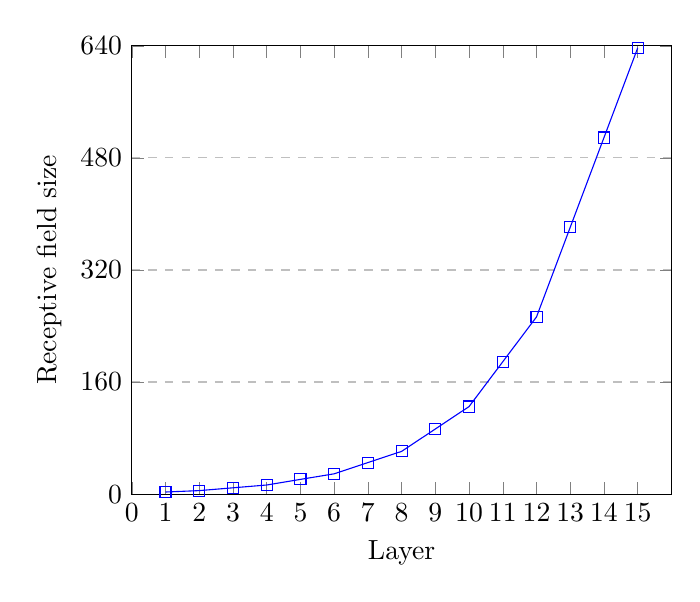
\begin{tikzpicture}
		\begin{axis}[
		%title={Receptive field vs Layer},
		xlabel={Layer},
		ylabel={Receptive field size},
		xmin=0, xmax=16,
		ymin=0, ymax=640,
		xtick={0,1,2,3,4,5,6,7,8,9,10,11,12,13,14,15},
		ytick={0,160,320,480,640},
		legend pos=north west,
		ymajorgrids=true,
		grid style=dashed,
		]
		
		\addplot[
		color=blue,
		mark=square,
		]
		coordinates {
			(1,3)(2,5)(3,9)(4,13)(5,21)(6,29)(7,45)(8,61)(9,93)
			(10,125)(11,189)(12,253)(13,381)(14,509)(15,637)
		};
		%\legend{CuSO$_4\cdot$5H$_2$O}
		
		\end{axis}
	\end{tikzpicture}
\end{document}
